\documentclass{article}
\usepackage{blindtext}
\usepackage[utf8]{inputenc}
\usepackage{amsmath,bm}
\usepackage{amstext}
\usepackage{amsfonts}
\usepackage{amsmath}
\usepackage{graphicx}
\title{Introduction to Machine Learning\\Homework 1}
\author{181860066 Niu Mingyang}
\date{2020.10.1}
\begin{document}
\maketitle

\section{[20pts] Basic review of probability}
The probability distribution of random variable $X$ follows:\\
\begin{equation}
f_X(x)=\begin{cases}
\frac{1}{2} & 0<x<1;\\
\frac{1}{6} & 2<x<5;\\
0 & \text{otherwise}.
\end{cases}
\end{equation} 
(1) [5pts] Please give the cumulative distribution function $F_X(x)$ for X;\\ \\
\begin{equation}
    F_X(x)=\int_{-\infty}^x f_X(x)=\begin{cases}
        0 & x\leq0;\\ 
        \frac{x}{2} & 0<x\leq1;\\
        \frac{1}{2} & 1<x\leq2;\\
        \frac{x+1}{6} & 2<x\leq5;\\
        1 & x>5.
        \end{cases} 
\end{equation}
\\ \\ 
(2) [5pts] Define random variable $Y$ as $Y=1/(X^2)$, please give the probability density function $f_Y(y)$ for $Y$;\\ \\
\begin{equation}
\begin{aligned}
    F_Y(y)&=P(Y \leq y)\\&=P(1/(X^2) \leq y)\\&=P(X \geq 1/\sqrt{y})\\&=1-P(X \leq 1/\sqrt{y})\\&=1-F_X(1/\sqrt{y})
    \\&=\begin{cases}
        0 & 0 \leq y<\frac{1}{25};\\ 
        \frac{5}{6} - \frac{1}{6\sqrt{y}} & \frac{1}{25} \leq y < \frac{1}{4};\\
        \frac{1}{2} & \frac{1}{4} \leq x < 1;\\
        1-\frac{1}{2\sqrt{y}} & x \geq 1.
    \end{cases}
\end{aligned}
\end{equation}
\begin{equation}
    f_Y(y)=F_Y'(y)=\begin{cases}
        \frac{1}{12} y^{-\frac{3}{2}} & \frac{1}{25} \leq y < \frac{1}{4};\\
        \frac{1}{4} y^{-\frac{3}{2}} & x \geq 1;\\
        0 & \text{otherwise}.
    \end{cases}
\end{equation}
\\ \\
(3) [10pts] For some random non-negative random variable Z, please prove the following two formulations are equivalent:\\
\begin{equation}
\mathbb{E}[Z]=\int^\infty_{z=0} z f(z)\mathrm{d}z,
\end{equation}
\begin{equation}
\mathbb{E}[Z]=\int^\infty_{z=0} \mathrm{Pr}[Z\geq z]\mathrm{d}z,
\end{equation}
Meantime, please calculate the expectation of random variable $X$ and $Y$ by these two expectation formulations to verify your proof.
\\ \\because Z is non-negative random varible,
\begin{equation}
\begin{aligned}
\mathbb{E}[Z]&=\int^\infty_{-\infty} z f(z)\mathrm{d}z=\int^\infty_{z=0} z f(z)\mathrm{d}z, 
\\\mathbb{E}[Z]&=\int^\infty_{z=0} z f(z)\mathrm{d}z
\\&=\int^\infty_{z=0} z \mathrm{d}F(z)
\\&=\int^\infty_{z=0} z \mathrm{d}(1-\mathrm{Pr}[Z\geq z])
\\&=-\int^\infty_{z=0} z \mathrm{d}\mathrm{Pr}[Z\geq z]
\\&=\int^\infty_{z=0} \mathrm{Pr}[Z\geq z]\mathrm{d}z - z\mathrm{Pr}[Z\geq z]{\mid}_0^{\infty}
\\&=\int^\infty_{z=0} \mathrm{Pr}[Z\geq z]\mathrm{d}z
\end{aligned}
\end{equation}

\section{[15pts] Probability Transition}

(1) [5pts] Suppose P(rain today) = 0.30, P(rain tomorrow) = 0.60,
P(rain today and tomorrow) = 0.25. Given that it rains today, what
is the probability it will rain tomorrow?\\\\
\begin{equation}
\begin{aligned}
    P(\text{rain tomorrow}|\text{rain today})&=\frac{P(\text{rain today and tomorrow})}{P(\text{rain today})}
    \\&=\frac{0.25}{0.3}=\frac{5}{6}
\end{aligned}
\end{equation}
\\\\
(2) [5pts] Give a formula for $P(G | \neg H)$ in terms of $P(G)$,
$P(H)$ and $P(G \wedge H)$ only.  Here $H$ and $G$ are boolean random variables.\\ \\
\begin{equation}
    P(G | \neg H) = \frac{P(G \wedge \neg H)}{P(\neg H)}=\frac{P(G)-P(G \wedge H)}{1-P(H)}
\end{equation}
\\\\
(3) [5pts] A box contains {\it w} white balls and {\it b} black
balls. A ball is chosen at random. The ball is then replaced,
along with {\it d} more balls of the same color (as the chosen
ball). Then another ball is drawn at random from the box. Show
that the probability that the second ball is white does not depend
on {\it d}.  \\\\
\begin{equation}
\begin{aligned}
    P &= P(\text{white first time}) + P(\text{black first time})
    \\&=\frac{w}{w+b} \cdot \frac{w-1+d}{w+b-1+d} + \frac{b}{w+b} \cdot \frac{w}{w+b-1+d}
    \\&=\frac{w}{(w+b)(w+b-1+d)} \cdot (w-1+d+b)
    \\&=\frac{w}{w+b}
\end{aligned}
\end{equation}
so P does not depend on {\it d}.

\section{[20pts] Basic review of Linear Algebra}
Let $x = (\sqrt{3}, 1)^{\top}$ and $y = (1, \sqrt{3})^{\top}$ be two vectors,\\\\
(1) [5pts] What is the value of $x_{\perp}$ where $x_{\perp}$ indicates the projection of $x$ onto $y$. \\\\
\begin{equation}
    \lvert x_{\perp} \rvert = x \cdot \frac{y}{\lvert y \rvert}=(\sqrt{3}, 1)^{\top}\cdot(1, \sqrt{3})^{\top}\cdot\frac{1}{2}=\sqrt{3}
\end{equation}
\\\\
(2) [5pts] Prove that $y \perp (x - x_{\perp})$.\\\\
\begin{equation}
\begin{split}
    &x_{\perp}=\sqrt{3}\frac{y}{\lvert y \rvert}=\sqrt{3}\cdot(1, \sqrt{3})^{\top}\cdot\frac{1}{2}=(\frac{\sqrt{3}}{2}, \frac{3}{2})^{\top},
    \\&x-x_{\perp}=(\frac{\sqrt{3}}{2}, -\frac{1}{2})^{\top},
    \\&y\cdot(x-x_{\perp})=(1, \sqrt{3})^{\top}\cdot(\frac{\sqrt{3}}{2}, -\frac{1}{2})^{\top}=0
\end{split}
\end{equation}
so $y \perp (x - x_{\perp})$.
\\\\
(3) [10pts] Prove that for any $\lambda \in \mathbb{R}$, $\lvert| x - x_{\perp}\rvert| \leq \lvert| x - \lambda y \rvert|$ \\\\
\begin{equation}
\begin{aligned}
    &\lvert x-x_{\perp} \rvert=1,
    \\&x-\lambda y=(1, \sqrt{3})^{\top}-(\lambda, \sqrt{3}\lambda)^{\top}=(\sqrt{3}-\lambda, 1-\sqrt{3}\lambda)^{\top},
    \\&\lvert x-\lambda y \rvert=\sqrt{(\sqrt{3}-\lambda)^2+(1-\sqrt{3}\lambda)^2}
    =\sqrt{4\lambda^2-4\sqrt{3}\lambda+4}=\sqrt{4(\lambda-\frac{\sqrt{3}}{2})^2+1}
    \geq 1.
\end{aligned}
\end{equation}
so $\lvert| x - x_{\perp}\rvert| \leq \lvert| x - \lambda y \rvert|$.

\section{[20pts] Hypothesis Testing}
A coin was tossed for $50$ times and it got $35$ heads, please determine that \emph{if the coin is biased for heads} with $\alpha = 0.05$.\\\\
\begin{equation}
    H_0:EX=0.5 \quad H_1:EX\neq0.5
\end{equation}
rejection region:$\lvert \bar{X}-\mu_0 \rvert>\sqrt{\frac{DX}{n\alpha}}$.\\
from sample:$\lvert \bar{X}-\mu_0 \rvert=\lvert \frac{35}{50}-0.5 \rvert=0.2$,
$\sqrt{\frac{DX}{n\alpha}}=\sqrt{\frac{0.25}{100\cdot0.05}}=\frac{\sqrt{5}}{10}$.\\
so$\lvert \bar{X}-\mu_0 \rvert<\sqrt{\frac{DX}{n\alpha}}$,the coin is not biased for heads.

\section{[25pts] Performance Measures}
We have a set of samples that we wish to classify in one of two classes and a ground truth class of each sample (denoted as 0 and 1). For each example a classifier gives us a score (score closer to 0 means class 0, score closer to 1 means class 1). Below are the results of two classifiers ($C_1$ and $C_2$) for 8 samples,their ground truth values ($y$) and the score values for both classifiers ($y_{C_1}$ and $y_{C_2}$).
\begin{table}[htbp]
    \centering
    \begin{tabular}{c|cccccccc}
        \hline
        $y$ & 1 & 0 & 1 & 1 & 1 & 0 & 0 & 0\\
        \hline
        $y_{C_1}$ & 0.6 & 0.31 & 0.58 & 0.22 & 0.4 & 0.51 & 0.2 & 0.33\\
        \hline
        $y_{C_2}$ & 0.04 & 0.1 & 0.68 & 0.24 & 0.32 & 0.12 & 0.8 & 0.51\\
        \hline
    \end{tabular}
\end{table}

\noindent{(1) [10pts] For the example above calculate and draw the ROC curves for classifier $C_1$ and $C_2$. Also calculate the area under the curve (AUC) for both classifiers.}\\\\
for $C_1$:\\
\begin{figure}
    \centering
    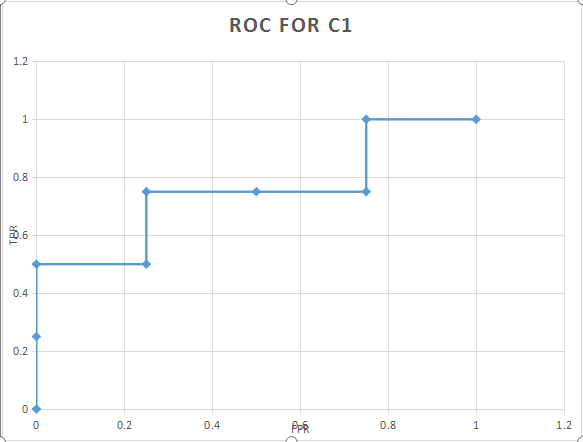
\includegraphics[width=.7\textwidth]{C:/Users/Administrator/Desktop/ROC for C1.png}
\end{figure}
\begin{equation}
    AUC=\frac{1}{4} \times \frac{1}{2} + \frac{1}{2} \times \frac{3}{4} + \frac{1}{4} \times 1=\frac{3}{4}
\end{equation}
for $C_2$:\\
\begin{figure}
    \centering
    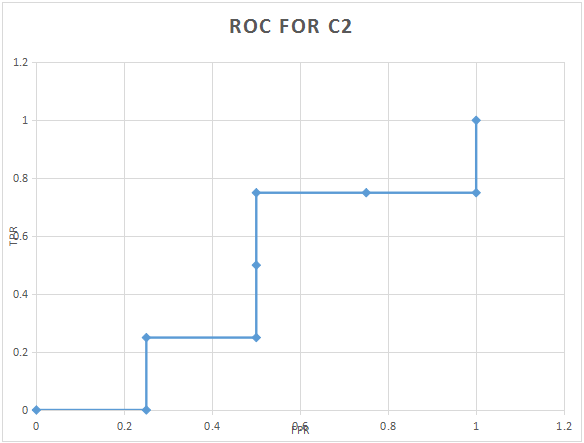
\includegraphics[width=.7\textwidth]{C:/Users/Administrator/Desktop/ROC for C2.png}
\end{figure}
\begin{equation}
    AUC=\frac{1}{4} \times 0 + \frac{1}{4} \times \frac{1}{4} + \frac{1}{2} \times \frac{3}{4}=\frac{7}{16}
\end{equation}
\\\\
(2) [15pts] For the classifier $C_1$ select a decision threshold $th_1 = 0.33$ which means that $C_1$ classifies a sample as class 1, if its score $y_{C_1} > th_1$, otherwise it classifies it as class 0. Use it to calculate the confusion matrix and the $F_1$ score. Do the same thing for the classifier $C_2$ using a threshold value $th_2 = 0.1$.\\\\
for $C_1$:\\
\begin{table}[htbp]
    \centering
    \begin{tabular}{c|cccccccc}
        \hline
        $\text{reality}/\text{prediction}$ & 1 & 0\\
        \hline
        1 & 3 & 1\\
        \hline
        0 & 1 & 3\\
        \hline
    \end{tabular}
\end{table}
\begin{equation}
    F1=\frac{2 \cdot TP}{m+TP-TN}=\frac{2 \cdot 3}{8+3-3}=0.75
\end{equation}
for $C_2$:\\
\begin{table}[htbp]
    \centering
    \begin{tabular}{c|cccccccc}
        \hline
        $\text{reality}/\text{prediction}$ & 1 & 0\\
        \hline
        1 & 3 & 1\\
        \hline
        0 & 3 & 1\\
        \hline
    \end{tabular}
\end{table}
\begin{equation}
    F1=\frac{2 \cdot TP}{m+TP-TN}=\frac{2 \cdot 3}{8+3-1}=0.6
\end{equation}
\end{document}